\documentclass[floatfix]{article}
\usepackage[utf8x]{inputenc}
\usepackage[pdftex]{graphicx}
\usepackage{mathpazo} 
\usepackage{amsmath}
\usepackage{amsfonts}
\usepackage{amssymb}
\usepackage{braket}
\usepackage{dsfont}
\usepackage[pdftex]{hyperref}   
\usepackage{siunitx}
\usepackage{bbm, dsfont}
\usepackage[font=small]{caption}
\usepackage[margin=1in]{geometry}
\usepackage{float}
\usepackage{tikz}
\usetikzlibrary{arrows,shapes,trees}


\newcommand{\id}{\mathbb{1}}


\graphicspath{{images/},{figures/}}

\title{Nested environments}
\author{Eduardo Villase\~nor}
\date{\today}

\begin{document}
\maketitle



\section{Introduction}

We are interested in studying a central system of a spin 1/2 that has a interaction to a nested  
environment. To accomplish this, we simulate the environments using ensembles of random matrices,
specifically we use the Gaussian unitary ensemble.

The Hamiltonian for the complete system is as follows:
\begin{equation}
H=H_c+ H_{ee}+\lambda V_{\text{ce}},
\end{equation}
with
\begin{equation}\label{general_model}
 H_c=\sigma_z \otimes \id_{\text{e}} \otimes \id_{\text{e}'},
\end{equation}
 \begin{equation}
  H_{\text{ee}}=\id_{\text{c}}  \otimes U_{\text{GUE}}^{N_e \times N_e'},
 \end{equation}
 \begin{equation}
V_{\text{ce}}= U_{\text{GUE}}^{2 \times N_e} \otimes \id_{\text{e}'}.
 \end{equation}
where $N_e$ and $N_e'$ denote the dimensions of the near and far environments respectively.

To perform time evolutions we take the initial state as follows:
$$  \Ket{\psi} = \Ket{\psi_c} \otimes \Ket{\psi_e^{\text{Random}}} \otimes \Ket{\psi_{e'}^{\text{Random}}}$$
where $\psi_c = \frac{1}{\sqrt{2}}( \Ket{0} + \Ket{1})$.





\section{First Results}

For the first results we use compute the purity of the central system. In all cases we averaged the calculations
50 times, for different random matrices and initial random states, in order to take into account the effects of the ensembles.
\begin{figure}[H] 
 \centering
 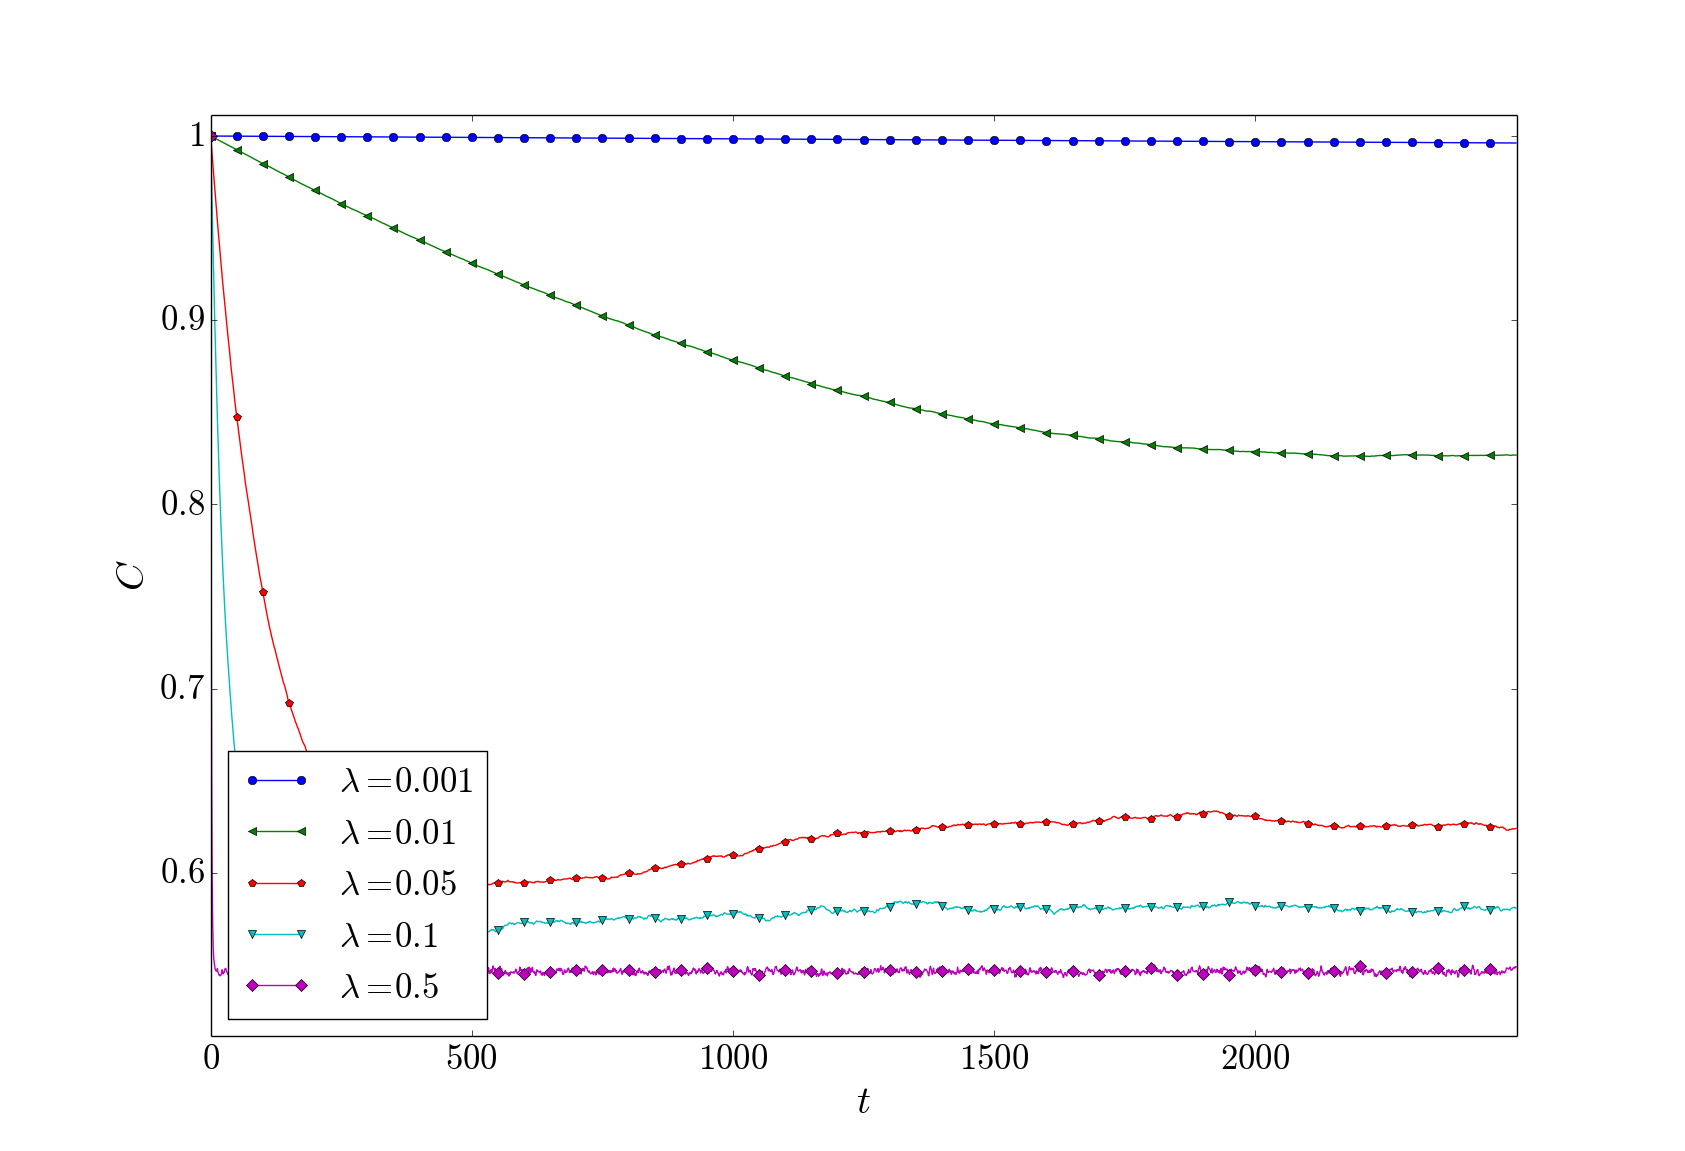
\includegraphics[width=.8\textwidth]{grafica1.png}
 \caption{Purity as a function of time for different values of $\lambda$. Here the dimensions of the environments
 are $N_e=2^3$ and $N_e'=2^6$.}
\end{figure} 


\begin{figure}[H] 
 \centering
 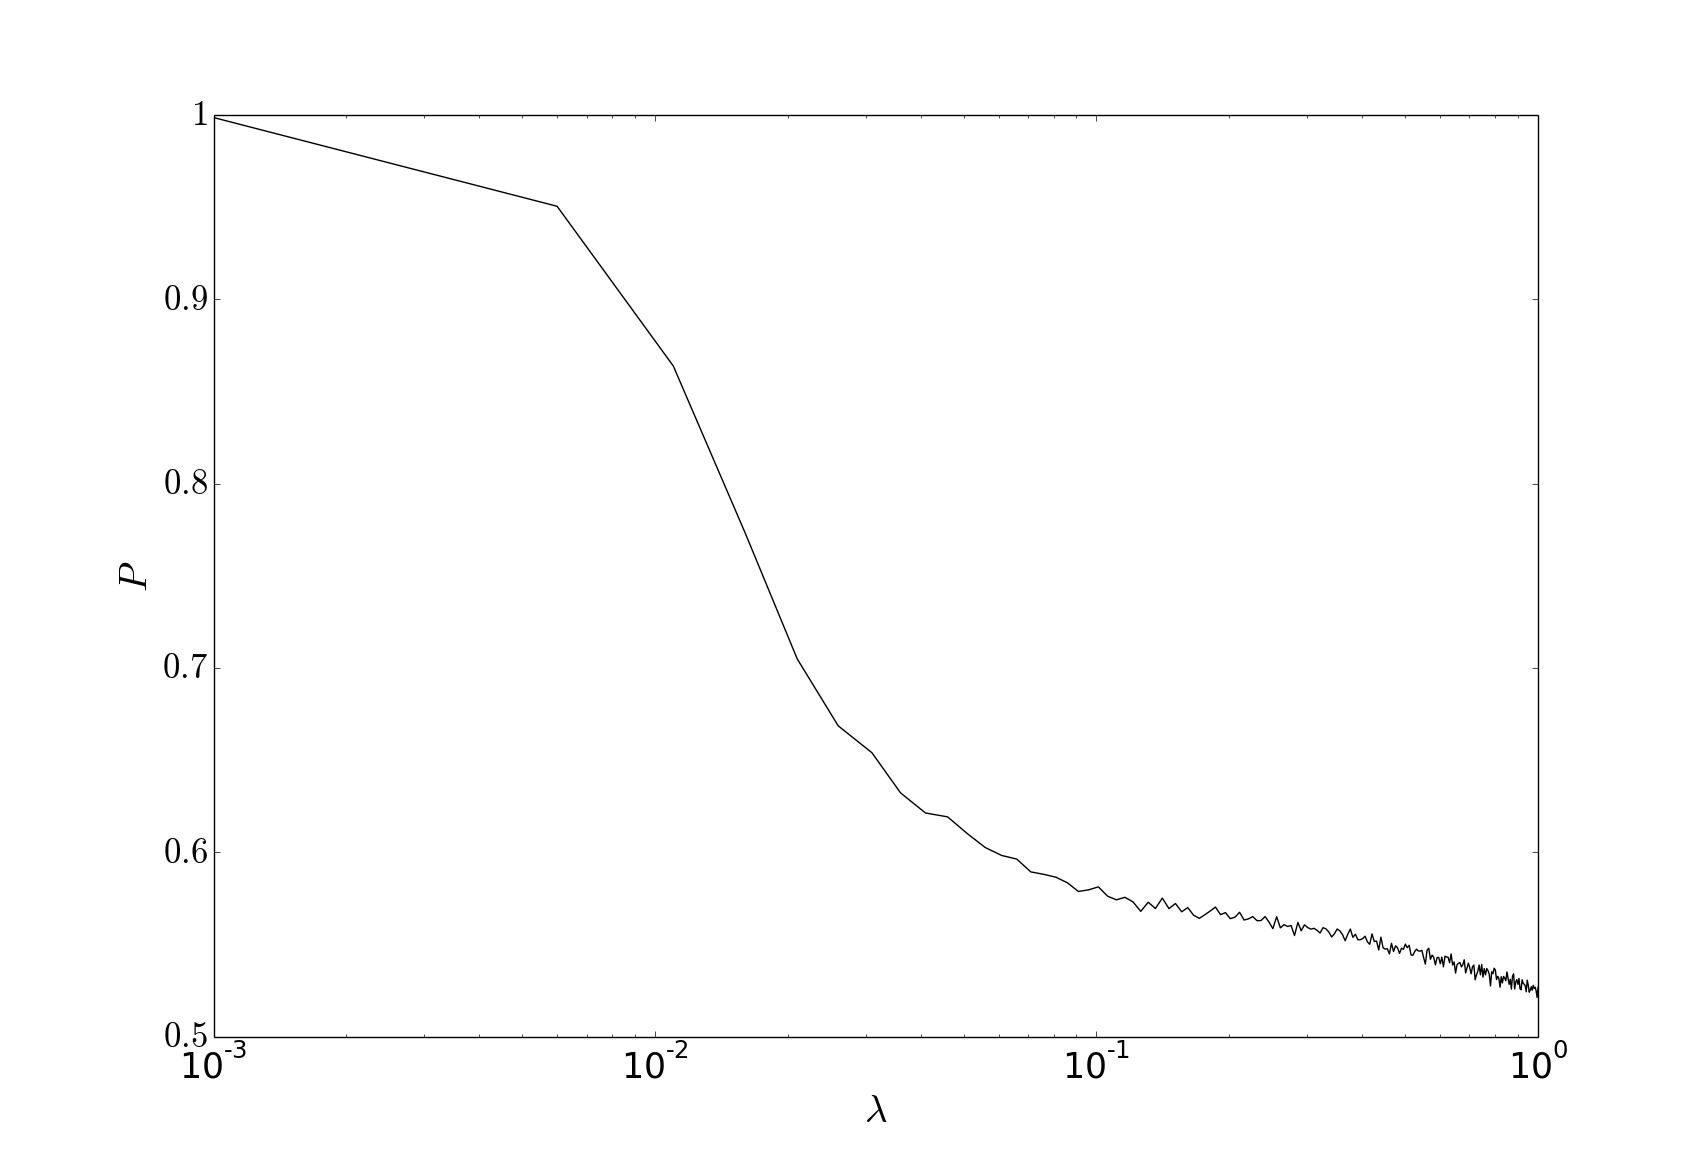
\includegraphics[width=.8\textwidth]{grafica2.png}
  \caption{ We plot the purity at the fixed time $t=1000$ as a function of $\lambda$. The dimensions of the environments
 are $N_e=2^3$ and $N_e'=2^6$.}
\end{figure} 


\begin{figure}[H]  
 \centering
 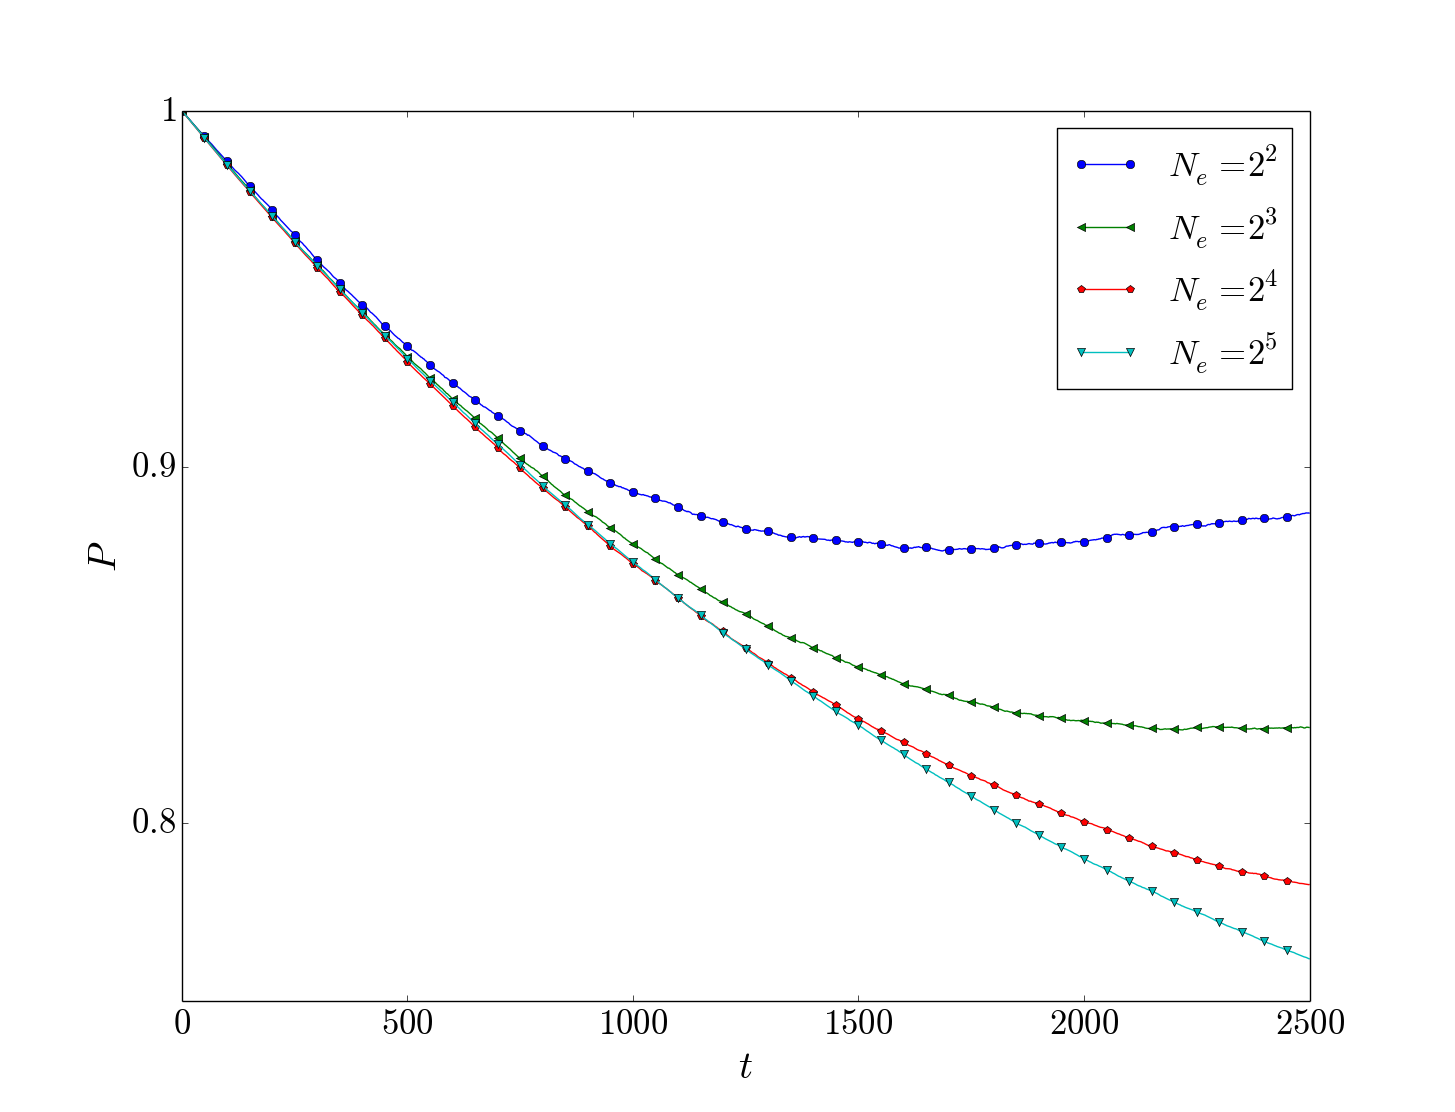
\includegraphics[width=.8\textwidth]{grafica4.png}
   \caption{ We plot the purity as a function of time, with the value $\lambda=0.01$ fixed. The dimension of the far environment
 is set to $N_e'=2^6$, where we vary the dimension of the near environment.}
\end{figure} 



\section{Two qubits as central system}

For the case when two qubits are the central system we must take the Hamiltonian $H_c$ as follows:
$$H_c=(\sigma_z \otimes \id_{2} + \id_{2}  \otimes \sigma_z) \otimes \id_{\text{e}} \otimes \id_{\text{e}'}.$$.
Additionally the initial state of the central system now corresponds to a Bell state, $\psi_c = \frac{1}{\sqrt{2}}( \Ket{00} + \Ket{11})$. 


\begin{figure}[H]  
 \centering
 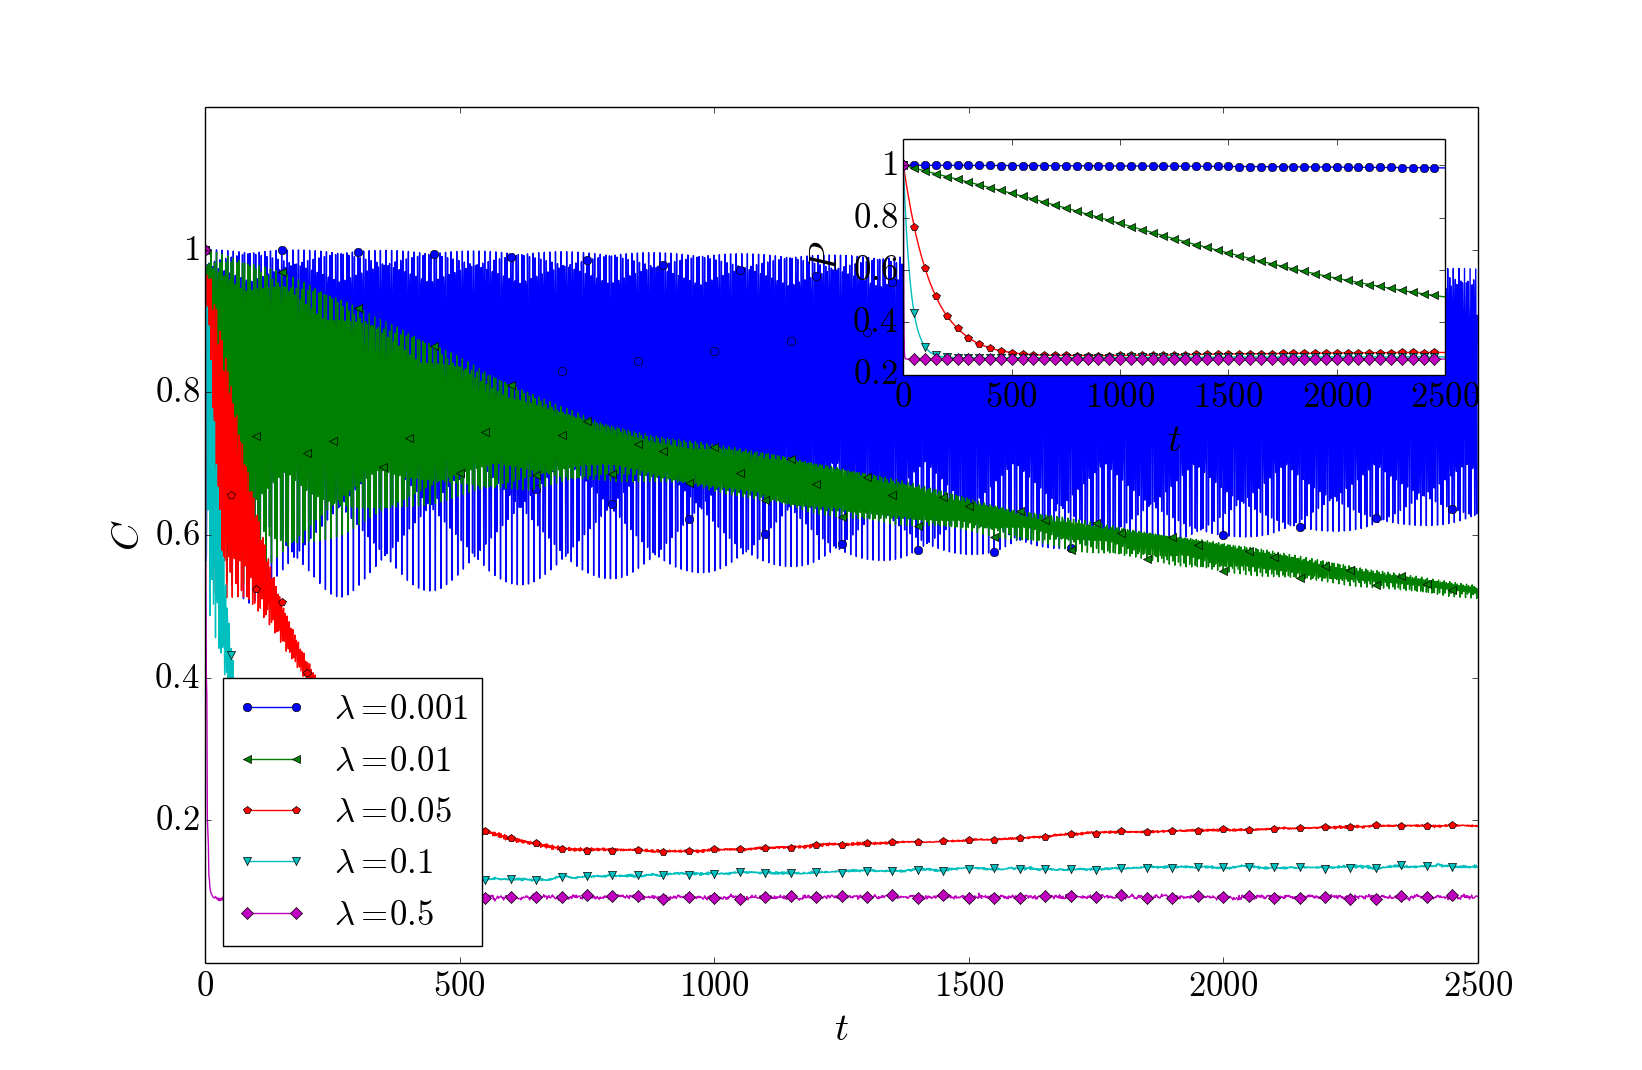
\includegraphics[width=.8\textwidth]{grafica3.png}
 \caption{Concurrence as a function of time for different values of $\lambda$. The inset show the purity.
 (NOTA: Es importante remarcar que en este caso ambos qubits interaccionan con el ambiente cercano, ya estoy
 calculando el caso en el que uno es observador).}
\end{figure} 




\end{document}
